\chapter{磁場中でのPMTの動作確認(担当:井口)}\label{PMT}

\section{動機}
磁場中のポジトロニウムの寿命測定実験(本実験)では,2インチPMT(光電子増倍管)とトリガー用の3/8インチPMTを磁場中で使用する.PMTは一般に磁場中ではゲインが低下してしまうため,あらかじめ磁場中でPMTの動作を確認する必要がある.この章で述べる実験では,PMTを磁場中で使用した場合のゲインの変化を,$\gamma$線源のスペクトルを測定することで確認した.また鉄管でPMTを覆い同様の測定をおこなうことで磁場の遮蔽を試みた場合のゲインの変化を確認した.


\section{電磁石}
この実験では,本実験と同じ電磁石を用いる.2章でも述べたように、磁極の直径は100 mm,磁極間の距離は150 mmである。またこの章では、電磁石のN極からS極へ向かう方向を$z$方向とし,磁極間の中点を$z=0$ cmとする.さらに磁極の半径方向を$r$方向とし,磁極の中心を$r=0$ cmとする.
\begin{figure}[h!]
	\centering
	\includegraphics[width=13cm]{fig/iguchi/magnetfigure.pdf}
	\caption{電磁石図}
	\label{magfigure}
\end{figure}

\begin{figure}[h!]
	\centering
	\includegraphics[width=8cm]{fig/iguchi/magnetphoto.pdf}
	\caption{電磁石の写真}
	\label{magphoto}
\end{figure}

\newpage
はじめに電磁石に定格6.0 Aの電流を流し,ガウスメータを用いて,$z=0$ cmでの$z$方向の磁場の強さと$r$方向の関係を測定した.電磁石のコイルの半径は185 mmであるため、磁場の強い$r=20$ ㎝以下は2 cm毎、磁場の大きさの変化が少ない$r=20$ cm以上からは5 cm毎に測定した。
磁極の中心の磁場の大きさは約90 mTだった.
\begin{figure}[h!]
	\centering
	\includegraphics[width=15cm]{fig/iguchi/maggraph01.pdf}
	\caption{$z$方向磁場の$r$依存}
	\label{maggraph01}
\end{figure}

%\begin{itemize}
 %      \item 電磁石のN極からS極の方向を$z$方向とし,磁極間の中点を$z=0$ cmとする.
  %     \item 磁極の半径方向を$r$方向とし,磁極の中心を$r=0$ cmとする.
%\end{itemize}

\newpage
\section{2インチPMT}
今回の実験で使用した2インチPMTは、本実験でも使用する予定である浜松ホトニクス製の光電子増倍管アッセンブリH6410\cite{pmtH6410}である。

\begin{table}[htb]
	\centering
	 \begin{tabular}{cccccccc}\hline
	型名& 管径 & 外径 & 長さ & 最大電圧 & 印加電圧 & ゲイン & ダイノード構造 \\ \hline \hline
	H6410 & 2 インチ & 60 mm & 200 mm & -2000 V & -1850 V & $3.0\times10{^{6}}$ &ラインフォーカス型/10段 \\ \hline
	\end{tabular}
	  \caption{2インチPMTデータ表}
\end{table}

\begin{figure}[h]
  \begin{center}
    \begin{tabular}{c}
    %1
      \begin{minipage}[t]{0.5\hsize}    
        \begin{center}
          \includegraphics[width=6.5cm]{fig/iguchi/PMTphoto.jpg}
	\hspace{1cm}[1]2インチPMT H6410
     \end{center}
    \end{minipage}
    %2
      \begin{minipage}[t]{0.5\hsize}    
        \begin{center}
          \includegraphics[width=6.5cm]{fig/iguchi/PMTinner.pdf}
         \hspace{2cm}[2]ラインフォーカス型の内部構造
         \end{center}
        \end{minipage}
     
     \end{tabular}
     \label{PMT12}
    \end{center}
 \end{figure}

PMTを磁場中で使用すると,光電子がPMT内部を進む間にローレンツ力を受けて軌道が曲がり,ダイノードに届かなくなることでゲインが著しく低下する.

\section{2インチPMTの測定方法と装置図}
2インチPMTの光電面にNaI(Tl)シンチレータ(直径:57 mm,長さ:58 mm)\ref{NaIscinti}を取り付け,$\ce{^{60}Co}$と光電面の距離を70 mmに固定し,磁場なしの場合と磁場ありの場合でゲインを測定した.また磁極の中心からPMTの光電面までの距離を$r$方向の距離とする.
 
\begin{figure}[h!]
  \begin{center}
    \begin{tabular}{c}
    %1
      \begin{minipage}[h]{0.5\hsize}    
        \begin{center}
          \includegraphics[width=6.5cm]{fig/iguchi/2inchsokutei.pdf}
	\hspace{2cm}[1]測定装置
     \end{center}
    \end{minipage}
    %2
      \begin{minipage}[h]{0.5\hsize}    
        \begin{center}
          \includegraphics[width=6.5cm]{fig/iguchi/soutizu1.pdf}
         \hspace{2cm}[2]装置図
         \end{center}
        \end{minipage}
     
     \end{tabular}
     \label{souchi}
    \end{center}
 \end{figure}

\begin{figure}[h]
	\centering
	\includegraphics[width=5cm]{fig/iguchi/NaIscinti.jpg}
	\caption{NaI(Tl)シンチレータ}
	\label{NaIscinti}
\end{figure}

%\begin{table}[h]
%	\centering
%	 \begin{tabular}{lcc}\hline
%	種類& 直径 & 長さ \\ \hline \hline
%	NaI(Tl)シンチレータ & 57 mm & 58 mm \\ \hline
%	\end{tabular}
%	  \caption{NaI(Tl)シンチレータデータ表}
%\end{table}     
 
\subsection{2インチPMTの測定結果}

\begin{figure}[h]
	\centering
	\includegraphics[angle=-90,width=10cm]{fig/iguchi/121550on.pdf}
	\caption{$r=50$ cmのヒストグラム}
	\label{hist50}
\end{figure}

\begin{figure}[h]
	\centering
	\includegraphics[angle=-90,width=10cm]{fig/iguchi/121635on.pdf}
	\caption{$r=35$ cmのヒストグラム}
	\label{hist35}
\end{figure}

縦軸にPMTのゲイン,横軸にr方向の距離をとる.縦軸は磁場なしの場合のゲインで規格化した.磁場なしと$r=50,45$ cmのときは$\ce{^{60}Co}$の2つのピーク(1.17 MeV,1.33 MeV)が見える.$r=35$ cm(1.22 mT)ではゲインが大幅に低下した.$r=25$ cm(4.82 mT)では信号が完全に消失した.
スペクトルのピークはガウシアンと一次関数でフィットした.$\ce{^{60}Co}$の2つのピークの形は同じだと考えて,ノイズは一次関数で表せると考えた.

\begin{figure}[t]
	\centering
		\includegraphics[angle=-90,width=10cm]{fig/iguchi/plot2inchPMT.pdf}
	\caption{2インチPMTの磁場中のゲイン変化}
	\label{plot2inchoff}
\end{figure}

この結果からPMTは$r=35$ cm,$z$方向磁場の強さが1.22 mTで使用出来なくなる.

\section{2インチPMTの測定方法と装置図(鉄管あり)}
磁場を遮蔽するため,PMTを鉄管に挿入して先述と同様の測定を行った.
\begin{table}[h]
	\centering
	 \begin{tabular}{cccc} \hline
		素材 & 外径 & 内径 & 長さ \\ \hline \hline
		軟鉄 & 76.3 mm & 62.3 mm & 270 mm \\ \hline
	\end{tabular}
	  \caption{鉄管データ表}
	  \label{ironpipedata}
\end{table}

磁力線が鉄管端から内部に入り込む可能性を考慮して,鉄管端とPMTの光電面との距離が70 mmになるように取り付けた.
鉄は強磁性体であり,磁力線は磁化しやすい物質に吸収されるため,鉄管内部は磁力線が通らなくなり,磁場が遮蔽される.

\begin{figure}[tbp]
  \begin{center}
    \begin{tabular}{c}
    %1
      \begin{minipage}[h]{0.5\hsize}    
        \begin{center}
          \includegraphics[width=6.5cm]{fig/iguchi/PMTinFe.pdf}
	\hspace{3cm}[1]鉄管内部図
     \end{center}
    \end{minipage}
    %2
      \begin{minipage}[h]{0.5\hsize}    
        \begin{center}
          \includegraphics[width=6.5cm]{fig/iguchi/jibakyusyu.jpg}
         \hspace{3cm}[2]磁性体によって吸収される磁場
         \end{center}
        \end{minipage}
     
     \end{tabular}
    \end{center}
   \end{figure}
   

\begin{figure}[h]
	\centering
		\includegraphics[width=7cm]{fig/iguchi/2inchinFe.jpg}
	\caption{測定装置(鉄管あり)}
	\label{2inchinFe}
\end{figure}

%\begin{figure}[h]
	%\centering
		%\includegraphics[width=7cm]{fig/iguchi/ironpipe.jpg}
	%\caption{鉄管}
	%\label{ironpipe}
%\end{figure}



\subsection{2インチPMTの測定結果(鉄管あり)}

\begin{figure}[h]
	\centering
		\includegraphics[clip,angle=-90,width=10cm]{fig/iguchi/122350fe.pdf}
	\caption{$r=50$ cm(鉄管あり)のヒストグラム}
	\label{hist50fe}
\end{figure}
\begin{figure}[h]
	\centering
		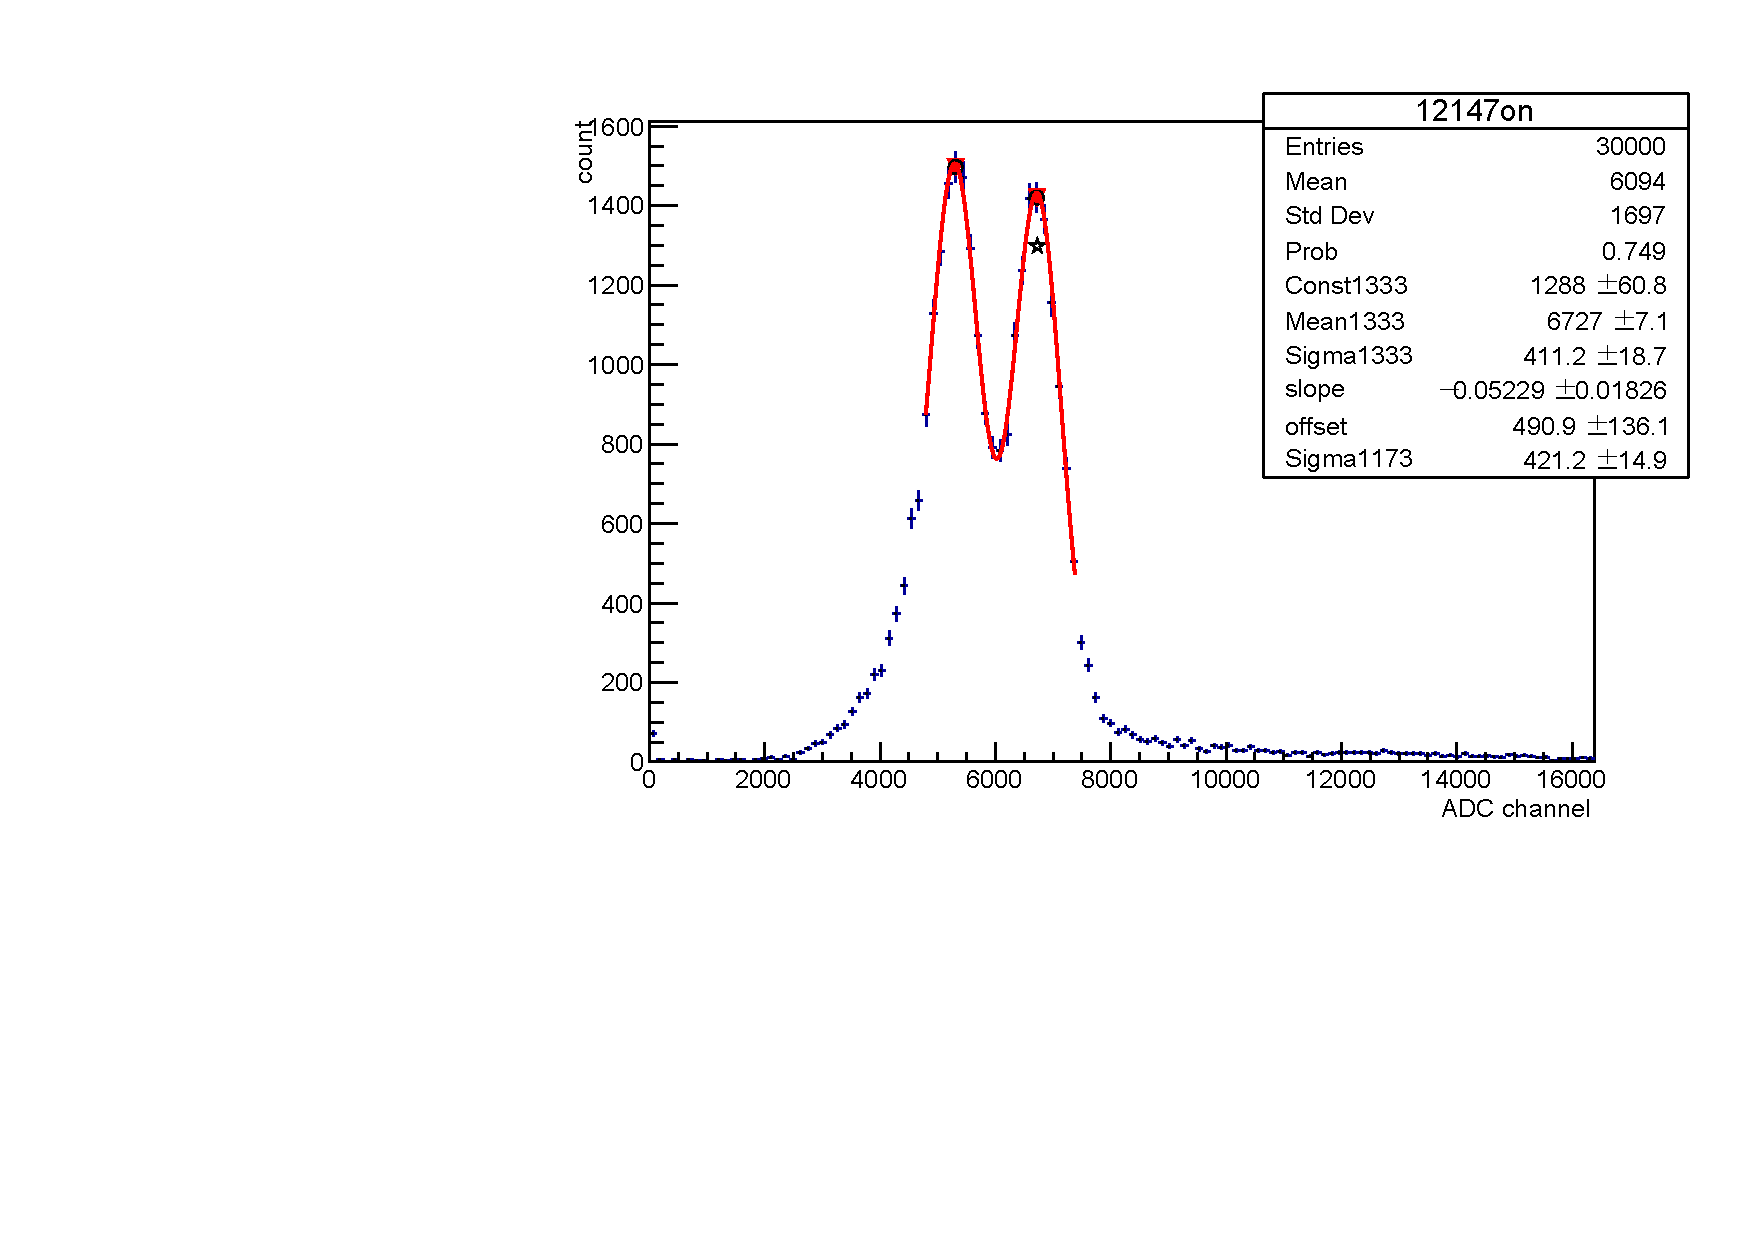
\includegraphics[clip,angle=-90,width=10cm]{fig/iguchi/12147on.pdf}
	\caption{$r=7$ cm(鉄管あり)のヒストグラム}
	\label{hist7fe}
\end{figure}

\begin{figure}[h]
	\centering
		\includegraphics[angle=-90,width=10cm]{fig/iguchi/bigPMTfit.pdf}
	\caption{2インチPMTでの磁場中のゲイン変化(鉄管あり)}
	\label{bigPMTfit}
\end{figure}
鉄管なしの場合と同様にゲインを規格化し,同様の手法でピークをフィットした.$r=20$ cmまでゲインがほとんど低下しない.$r=20$ cm以下ではややゲインが低下するが、$r=7$ cmまで2つのピークを見ることができる.
本実験において2インチPMTは$r=12$ cmに設置する予定なので,鉄管に挿入し磁場を遮蔽することで,本実験でも使用可能である.


\section{3/8インチPMT}
3/8インチPMT\cite{pmtH3164-10}は,本実験ではトリガー用に使用されるため,2章の図\ref{fig:device2}のように2インチPMTより磁極に近い位置に,光電面が$r=1.5$ cmとなるように設置される.

\begin{figure}[H]
	\centering
		\includegraphics[width=10cm]{fig/iguchi/miniPMT.jpg}
	\caption{3/8インチPMT H3164-10}
	\label{3/8inch}
\end{figure}

\begin{table}[h]
	\centering
	
	  \begin{tabular}{cccccccc} \hline
		型名& 管径 & 外径 & 長さ & 最大電圧 & 印加電圧 & ゲイン & ダイノード構造 \\ \hline \hline
		H3164-10 & 3/8 インチ & 10.5 ㎜ & 45 mm & -1500 V & -1400 V & $1.0\times10{^{6}}$ &ラインフォーカス型/8段 \\ \hline
	\end{tabular}
	  \caption{3/8インチPMTデータ表}
	  \label{3/8inchPMT}
\end{table}


\subsection{3/8インチPMTの測定方法と装置図}

先述の実験と同様の方法で,$\ce{^{22}Na}$と3/8インチPMTの光電面との距離を100 mmで固定し,鉄管に入れた場合と入れない場合でゲインを測定した.
3/8インチPMTはダークカレントが多く線源のスペクトルが見えにくかったため,一つのNaIシンチレータに二つの3/8インチPMTを取り付け,それらの信号を同時計測することでダークカレントを落とした.


\begin{figure}[h]
  \begin{center}
    \begin{tabular}{c}
    %1
      \begin{minipage}[h]{0.4\hsize}    
        \begin{center}
          \includegraphics[width=6.5cm]{fig/iguchi/PPMT.jpg}
	\hspace{3cm}[1]3/8インチPMTのコインシデンス
     \end{center}
    \end{minipage}
    %2
      \begin{minipage}[h]{0.6\hsize}    
        \begin{center}
          \includegraphics[width=10cm]{fig/iguchi/miniset.pdf}
         \hspace{3cm}[2]3/8インチPMTの装置図
         \end{center}
        \end{minipage}
     
     \end{tabular}
    \end{center}
   \end{figure}
   

また鉄管は2インチPMTの実験で用いたものと同一のものを使用し,線源はスペクトルのピークの位置がわかりやすい$\ce{^{22}Na}$を使用した.


\subsection{3/8インチPMTの測定結果}

\begin{figure}[h]
	\centering
		\includegraphics[angle=-90,width=10cm]{fig/iguchi/minicoout22.pdf}
	\caption{$r=22$ cmのヒストグラム(鉄管なし)}
	\label{histminicoout22}
\end{figure}

\begin{figure}[h]
	\centering
		\includegraphics[angle=-90,width=10cm]{fig/iguchi/minicoin22.pdf}
	\caption{$r=50$ cmのヒストグラム(鉄管あり)}
	\label{histminicoin22}
\end{figure}

\begin{figure}[h]
	\centering
		\includegraphics[angle=-90,width=10cm]{fig/iguchi/minicoin21.pdf}
	\caption{$r=6$ cmのヒストグラム(鉄管あり)}
	\label{histminicoin21}
\end{figure}

\begin{figure}[h]
	\centering
		\includegraphics[angle=-90,width=10cm]{fig/iguchi/miniPMTgainG.pdf}
	\caption{3/8インチPMTの磁場中でのゲイン変化}
	\label{miniPMTgainG}
\end{figure}

先述の実験と同様に,横軸にr方向の距離,縦軸にゲインをとった.縦軸は磁場なしで測定したときのゲインで規格化した.また1.275MeVのピークはガウシアン+二次関数でフィットした.鉄管に入れない場合,$r=30$ cm(2.36 mT)まではゲインが低下しないが,$r=25$ cm(4.82 mT)付近からゲインが低下し,$r=22$ cm(10 mT以下)でゲインが低下しピークが見えなくなった.

鉄管に入れた場合,$r=6$ cmまでゲインが低下せず,スペクトルのピークがはっきり見える.


\section{3/8インチPMTの測定結果と磁場シミュレーション}
測定結果から3/8インチPMTはコインシデンスを取り,鉄管に入れることで$r=6$ cmまで使用できることがわかった.
しかし本実験では,3/8インチPMTを外径21.7 mm,内径16.1 mmの鉄管に挿入し,3/8インチPMTを$r=1.5$ cmに設置する.また鉄管の端とPMT光電面の距離は5 mmである.

\begin{figure}[H]
	\centering
		\includegraphics[width=10cm]{fig/iguchi/honjikken.pdf}
	\caption{本実験でのセットアップ}
	\label{honjikken}
\end{figure}

本実験をおこなう前に,上の条件でも3/8インチPMTが使用出来るかを確認するため,磁場シミュレーションソフト(Femtet)を使用した.
電磁石の磁場をFemtetで再現し,本実験で3/8インチPMTを挿入する鉄管も同様に再現して,鉄管内部の磁場をシミュレーションした.

\subsection{磁場シミュレーション結果}
\begin{figure}[h]
	\centering
		\includegraphics[width=16cm]{fig/iguchi/magnetgraph2.pdf}
	\caption{femtetで再現した磁場と実測定した磁場}
	\label{magnetgraph2}
\end{figure}

グラフから確認できるように,femtetで再現した$z$方向磁場と実際の測定結果を比較すると,ほとんど一致していることからfemtetの磁場シュミレーションは妥当であることがわかる.
\begin{figure}[h]
	\centering
		\includegraphics[width=15cm]{fig/iguchi/maggraphinFe.pdf}
	\caption{femtetで再現した磁場(鉄管あり)}
	\label{maggraphinFe}
\end{figure}
鉄管内部の$z$方向磁場のシミュレーション結果から,本実験で3/8インチPMTの光電面が設置される$r=1.5$ cmでの磁場の強さは1.5 mTである.3/8インチPMTが使用可能であった$r=30$ cmでの磁場の強さは2.36 mT,使用不可能になった磁場の強さは約10 mTである.これらの結果を比較すると,シミュレーションで再現した鉄管内部の磁場の方が弱いため,3/8インチPMTは管径21.7 mmの鉄管に入れることで磁場中でも使用可能である.

\section{トリガー用PMT}
今までの実験で使用した3/8インチPMT\cite{pmtH3164-10}と四角型PMT(R2248)\cite{pmtR2248}は形状以外は同一である.よって2章で評価したSCtrigとして,どちらの型のPMTも使用可能であると結論付ける.

\ref{3/8inchPMT}

\begin{table}[h]
	\centering
	  \begin{tabular}{cccccccc} \hline
		型名& 管径 & 外径 & 長さ & 最大電圧 & 印加電圧 & ゲイン & ダイノード構造 \\ \hline \hline
		R2248 & 8 mm(角型) & 9.8 ㎜(角型)& 45 mm & -1500 V & - & $1.1\times10{^{6}}$ &ラインフォーカス型/8段 \\ \hline
	\end{tabular}
	  \caption{角型PMTデータ表}
\end{table}

\section{まとめ}
2インチPMTは鉄管に挿入し磁場を遮蔽することで$r=7$ cmまで使用可能であったため,本実験で設置する予定である$r=12$ cmでも鉄管に挿入することで使用可能である.また3/8インチPMTは2つのPMTを同時計測し鉄管に挿入することで$r=6$ cmまで使用可能であった.本実験でトリガー用PMTを挿入する鉄管の内部磁場を磁場シュミレーションで再現したものと,3/8インチPMTが使用可能であった磁場を比較した結果から,本実験で設置する予定である$r=1.5$ cmでも鉄管に挿入することで使用可能である.



